\documentclass[UTF8]{ctexart}


\usepackage{tipa}% 这里用于支持音标显示。此包必须在ctex宏包之前,否则会报错。


\usepackage{picinpar, graphicx} % 导入这个库后,就能支持插入表格
\graphicspath {{img_math/},{img2/}} %图片目录在当前目录的 img 和 img2文件夹下
\usepackage{float} 
\usepackage{subfigure}

\usepackage{algorithm, algorithmic, amsmath, amssymb,bm} % 支持数学公式输入
% \usepackage[fleqn]{amsmath} % 公式左对齐

\usepackage{ctex} % 支持字体加粗效果, 代码为 \textbf{加粗}


\usepackage{multicol} %用于实现在同一页中实现不同的分栏
\usepackage{wrapfig} %用于实现图文混排
\setlength{\parindent}{0pt} % 放在段首,之后的所有段落都将取消首行缩进

% 页面边距设置
\usepackage{geometry} %导入版面设置的宏包
\geometry{left=1.5cm, right=1.5cm, top=2cm, bottom=2cm} % 使用命令:\geometry{left=左边距,right=右边距,top=上边距,bottom=下边距}

\usepackage[skins]{tcolorbox} % 导入该包, 才能支持彩色文本框效果.  必须标注skin,才能使用shadow命令显示阴影

\usepackage{soul} % 支持英文高亮
\usepackage{xcolor} 
\newcommand{\mathcolorbox}[2]{\colorbox{#1}{$\displaystyle #2$}}

%支持修改公式中字体的颜色
\usepackage{xcolor}

% 支持直接打字希腊字母
%\usepackage{fontspec}
%\setmainfont{CMU Serif}


\title{导数 Derivative}




%------------------------------------------------------------



\begin{document}
	\tableofcontents % 生成目录
	\maketitle  %这行代码, 让你前面的 title, author, date生效




\part{什么是导数?}

某点处的``导数", 就是该点处``切线的斜率".

导数, 就是一个``极限值", 比如, y 在 点$x_0$ 处的导数, 就是:  $f'(x_0) = \lim_{\Delta x \to 0} \dfrac{\Delta y} {\Delta x} $


\begin{figure}[htbp]%调节图片位置,h:浮动;t:顶部;b:底部;p:当前位置
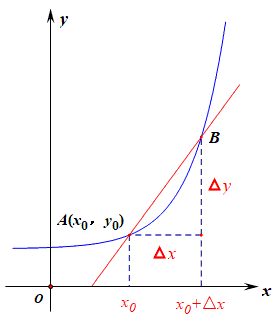
\includegraphics[width=0.25\textwidth]{/0023.png}
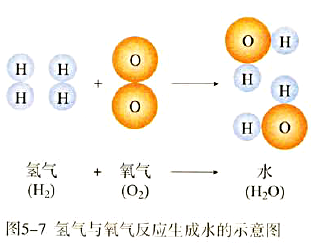
\includegraphics[width=0.25\textwidth]{/0024.png}
\end{figure}


可导, 就意味着图像很"光滑". 即图像没有"尖角"存在 (因为尖角处的左右导数不相等).

并且, 切线不能垂直于x轴. 如果切线是垂直于x轴的, 它的斜率就会是 +∞ 或 -∞了. \\



$x_0$ 点处的导数, 其实可以有下面4种写法来表示: 

(1) $y'|_{x=x_0}$

(2)  $f'(x_0)$

(3)  $\dfrac{dy} {dx}|_{x=x_0}$

(4) $\dfrac{d f(x)} {dx}|_{x=x_0}$ \\


``位置"的瞬时变化率(变换趋势, 能预测未来), 就是``速度". 所以速度是位置的导数. 

``速度"的瞬时变化率, 就是``加速度". 所以``加速度"是``速度"的导数. ``加速度"就是``位置"的二阶导.  \\

单侧导数, 就是从``某一侧"逼近某一x点时, 该点的切斜斜率.

所以, 左导数, 就是``从左侧向右"逼近了. 右导数, 就是``从右边向左"逼近了.

- 左导数 : $f_{-}^{’}\left( x_0 \right) =\lim_{x\rightarrow x_{0}^{-}}\dfrac{f\left( x \right) -f\left( x_0 \right)}{x-x_0}\\ $
- 右导数 : $f_{+}^{’}\left( x_0 \right) =\lim_{x\rightarrow x_{0}^{+}}\dfrac{f\left( x \right) -f\left( x_0 \right)}{x-x_0}\\ $


~\\
\hrule
~\\


\part{导数公式}

\section{常用的导数}



\subsection{$(\text{常数}C)' =0$}

常数不会变化, 自然没有``瞬时变化率"存在, 所以常数的导数就=0.





\subsection{$(x^n)'= n x^{n-1}$}

(1) 当指数 n=1时, 其导数=1. 

(2)  当 $n \textgreater 1$ 时, 其导数是 $ (x^n)' = n x^{n-1}$ \\

\begin{tcolorbox}[title = {例},boxrule={0.1em},colframe={black!10}, colback={black!3},colbacktitle={black!10},coltitle={black}]
求 $ y= \dfrac{1} {x}$  在 点(1/2, 2)处的切线的斜率(即导数), 并求出该切线的方程.

其导数是: $y'=\left( x^{-1} \right) '=-1x^{-1-1}=-1x^{-2}$

然后把 点(x=1/2, y=2) 代入进去, 得到: $y'\mid_{x=\frac{1}{2}}^{}=-1\left( \frac{1}{2} \right) ^{-2}=-4$  ← 这个数值, 就是 函数在点(1/2, 2)处的切线的斜率.

然后再套用直线的``点斜式方程" $y - y_1 = k(x- x_1)$

本例的切线即: $y-\underset{=2}{\underbrace{y_1}}=\underset{\text{即}y'=-4}{\underbrace{k}}\left( x-\underset{=\frac{1}{2}}{\underbrace{x_1}} \right)$
\end{tcolorbox}





\subsection{$\left( a^x \right) '=a^x\ln a$}

即直接后面跟个尾巴: ln a

例如, $(2^x)' = 2^x \ln 2$




\subsection{$(e^x)' = e^x \ln e = e^x$}

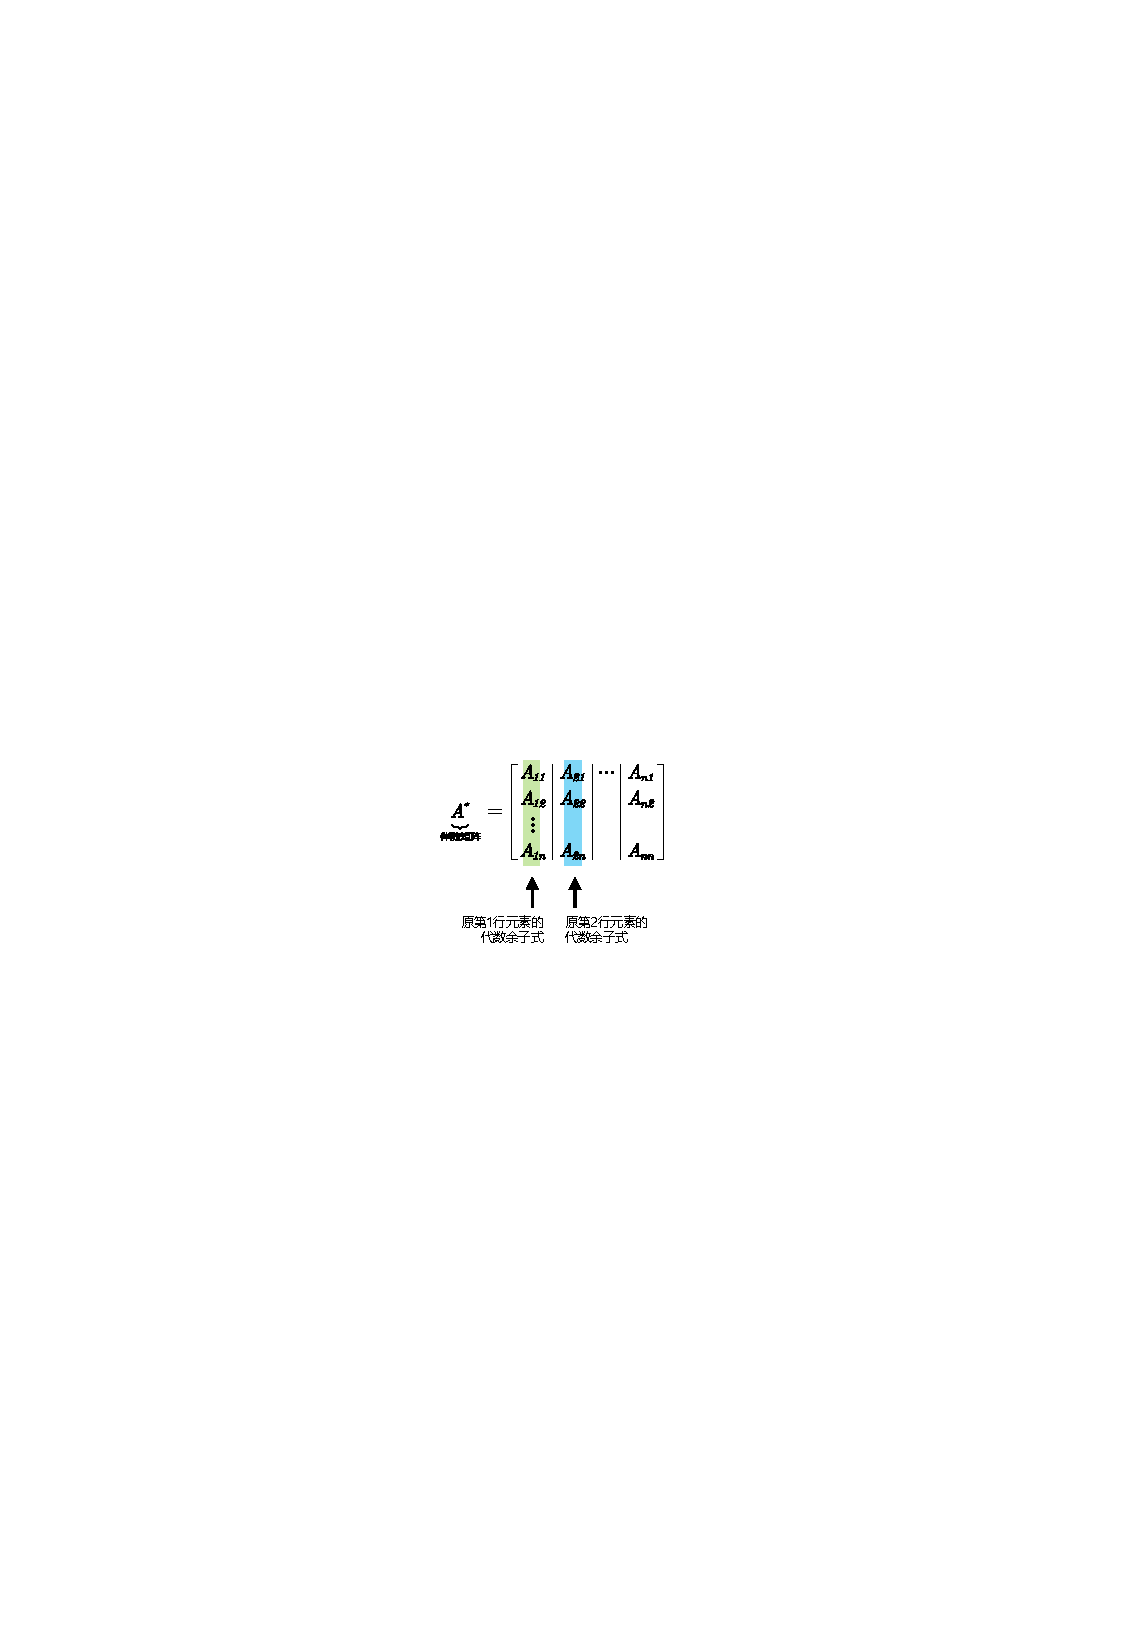
\includegraphics[width=0.4\textwidth]{/0025.pdf}




\subsection{$(\log_a x)' = \dfrac{1} {x \ln a}$}

即把 x 提到前面去, 把log 变成 ln, 整体再放在分母上. 分子为1. \\

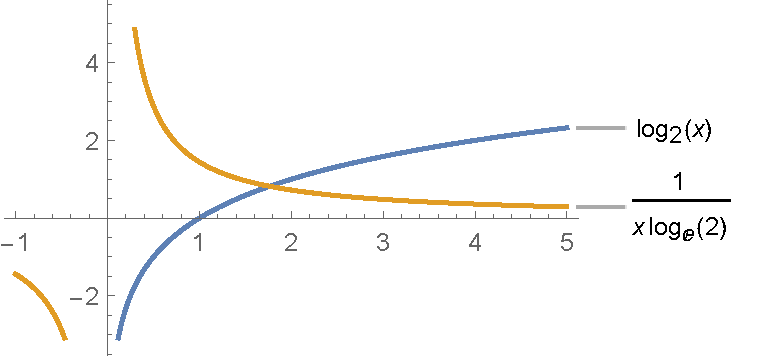
\includegraphics[width=0.4\textwidth]{/0026.pdf}



\subsection{$(\ln x)' = \dfrac{1} {x}$}

例如: 
$\left( \log _ex \right) '=\dfrac{1}{x\underset{=\log _ee=1}{\underbrace{\ln e}}}=\dfrac{1}{x}$



\section{反函数的导数 : $\boxed{[f^{-1}(y)]' = \dfrac{1} {\text{原函数的导数} f'(x)}}$}


反函数的导数, 和其原函数的导数, 呈``倒数关系". 

原函数是 y=f(x), 其反函数是 x=f(y), 则, 反函数的导数, 就是``原函数导数"的倒数. 


换言之, 原函数的导数是 $\dfrac{\varDelta y}{\varDelta x} $, , 则其反函数的导数就是  $\dfrac{1}{\frac{\varDelta y}{\varDelta x}}$.

``原函数"和``反函数", 它们``导数"的乘积 =1.

``原函数"与其``反函数"的图像, 是关于 y=x 对称的.




\section{三角函数的导数}

\subsection{$(\sin x)' = \cos x$}

\subsection{$(\cos x)' = -\sin x$}

\subsection{$(\tan x)' = \sec^2 x$}

\subsection{$(\cot x)' = -\csc^2 x$}

\subsection{$(\sec x)' = \sec x  \cdot \tan x$}

\subsection{ $(\csc x)' = - \csc x \cdot \cot x$}





\section{反三角函数的导数}

\subsection{$(\arcsin x)' = \dfrac{1} {\sqrt{1-x^2}}$}

\subsection{$(\arccos x)' = - \dfrac{1} {\sqrt{1-x^2}}$}

\subsection{$(\arctan x)' =  \dfrac{1} {1 + x^2}$}

\subsection{$(\operatorname{arccot}  x)' = - \dfrac{1} {1 + x^2}$}


~\\
\hrule
~\\


\part{求导的各种方法, 方法论}

\section{求导法则 : 和差积商}















\end{document}

